\documentclass[11pt]{article}

\usepackage[T1]{fontenc}
\usepackage[margin=1in]{geometry}
\usepackage{amsmath}
\usepackage{amssymb}
\usepackage{array}
\usepackage{booktabs}
\usepackage{graphicx}
\usepackage{hyperref}
\usepackage{multirow}
\usepackage{natbib}
\usepackage{enumitem}
\usepackage{xcolor}
\usepackage{microtype}

\setlength{\emergencystretch}{2em}

\graphicspath{{figures/}{../figures/}{paper/figures/}}

\newcommand{\ours}{\textnormal{\textsc{AgenticRAG-FP}}}
\newcommand{\dr}{\textnormal{\textsc{Doctor-RAG}}}
\newcommand{\pa}{\textnormal{\textsc{Propagation-Aware}}}
\newcommand{\lj}{\textnormal{\textsc{LLM-Judge}}}
\newcommand{\rb}{\textnormal{\textsc{Rule}}}
\newcommand{\sr}{\textnormal{\textsc{Suf-Regen}}}

\title{When Failures Propagate: Causal Failure Attribution\\
in Agentic Retrieval-Augmented Generation}

\author{
  Anonymous Authors \\
  \texttt{Research-AgenticRAG} \\
  \texttt{author emails}
}

\date{Draft generated from repository state on July 7, 2026}

\begin{document}
\maketitle

\begin{abstract}
Agentic retrieval-augmented generation (RAG) systems interleave retrieval,
reasoning, and answer generation across multiple hops.  This makes failures
difficult to diagnose: a retrieval error at hop 1 can surface only as a wrong
answer at hop 3, while later retrieval may partially repair the trajectory.  We
introduce \ours, a benchmark and experimental framework for causal failure
attribution in agentic RAG.  \ours{} logs hop-level traces, injects controlled
faults at specific hops, re-runs the downstream suffix of the agent trajectory,
and evaluates diagnosers against certified intervention labels.  Across
HotpotQA, MuSiQue, FRAMES, and CRAG, with Claude, GPT-4o-mini, and local/open
model conditions, we find a sharp identifiability collapse for coverage-based
post-hoc diagnosis: mean hop-1 attribution accuracy is 0.93, and after
decontaminating depth buckets (removing interventions that were silently
clamped to shallower hops), depth-2/3 accuracy is 0.00 in every rescorable
real-backbone condition (maximum single cell 0.03).  A counterfactual
propagation-aware localizer does not beat the best post-hoc baseline at
exact-hop localization on these structural faults (0 of 6 decontaminated deep
conditions).  We then introduce a
\emph{certified content-corruption} arm: instead of structurally corrupting
retrieval, we flip the answer-bearing or bridge fact inside otherwise-intact
documents and track the exact changed span, enabling a fully deterministic
generation-level evaluation (\emph{absorbed} / \emph{resisted} /
\emph{derailed}) with no LLM judge.  On content faults the coverage collapse
is total (1.00 at hop 1 to 0.00 at depth 2, pooled over four
backbone--dataset conditions) while the counterfactual localizer holds 0.67;
15\% of hop-1 corruptions are absorbed verbatim into the final answer, and
absorption is almost exclusively answer-shaped.  Suffix-regeneration probing
collapses on deep content faults for a mechanistic reason we identify ---
regenerating the suffix re-retrieves clean evidence and un-corrupts the fault
being probed --- while winning precisely the bridge-entity slice where frozen
local repair fails, motivating cascaded diagnosis.  These results establish
failure propagation as a first-class evaluation axis for agentic RAG and
characterize when local repair probes succeed.
\end{abstract}

\section{Introduction}

Retrieval-augmented generation (RAG) improves factual question answering by
conditioning generation on retrieved evidence rather than only on model
parameters \citep{lewis2020rag}.  Recent agentic variants make retrieval
iterative: a language model chooses sub-queries, observes retrieved documents,
and decides whether to search again or answer, in the style of ReAct-like
reasoning and acting \citep{yao2022react}.  This extra agency is useful for
multi-hop questions, but it fundamentally changes the failure mode.  The
observed error at the end of a trajectory is often not the root cause, and a
naive post-hoc diagnosis may point to the wrong hop or stage.

To see why, consider a three-hop RAG agent.  If hop 1 returns irrelevant
evidence, the agent may generate a drifted sub-query at hop 2, retrieve on a
wrong premise, and finally produce an ungrounded answer.  A post-hoc evaluator
inspecting the final trace can label the answer as wrong or identify a
late low-coverage hop, while entirely missing the earliest causal fault.
Conversely, some agents are surprisingly resilient: a noisy retrieval hop can be
corrected by a later retrieval, so the fault never manifests as an end-to-end
error at all.  Standard accuracy, retrieval recall, and answer correctness
conflate these three qualitatively different outcomes.

This paper studies \emph{failure propagation} as a first-class phenomenon.  We
ask: (C1) Can failures injected at a known hop be certified to propagate into a
final error, or does the agent self-correct?  (C2) If a failure propagates, can
a diagnoser recover its certified root cause as a function of propagation depth?
(C3) Does a counterfactual localizer improve on post-hoc coverage-based
methods?  (C4) When the fault is a \emph{content} error --- a wrong fact inside
otherwise-relevant documents --- rather than a structural retrieval error, does
any of this change, and can the downstream damage be measured deterministically?

To answer these questions, we introduce \ours, a provider-agnostic benchmark
that logs hop-level traces, injects controlled faults at specific hops and
stages, re-executes the downstream trajectory with the real agent, and evaluates
five classes of diagnosers against the known intervention labels.  The key
design requirement is \emph{causal certification}: because the benchmark
performs actual do-interventions and re-runs the agent, the resulting labels are
not post-hoc guesses but ground-truth causal assertions.

Our contributions are:
\begin{enumerate}[leftmargin=*]
  \item \textbf{A controlled live-intervention benchmark.}  \ours{} corrupts a
  trajectory prefix at hop $h$ and re-runs the downstream suffix with the same
  agent, producing certified intervention labels and genuine agent reactions rather
  than deterministic post-hoc edits.

  \item \textbf{An identifiability collapse finding (C2).}  A coverage-gated
  \dr-style baseline is nearly perfect at the injection hop but retains
  \emph{nothing} once the fault propagates: after actual-depth decontamination
  of the depth buckets, its accuracy at depths 2--3 is 0.00 in all ten
  nonempty deep cells across rescorable real-backbone conditions (max 0.03),
  versus a mean of 0.93 at hop 1.  An earlier uncorrected aggregate (0.30 at
  depth) turns out to have been an artifact of clamped shallow interventions
  contaminating deep buckets --- the collapse is total, not partial.

  \item \textbf{A mixed verdict on counterfactual localization (C3).}  Our \pa{}
  method beats the best post-hoc baseline in 0 of 6 decontaminated deep
  conditions on structural faults (an earlier 3-of-13 count reflected
  contaminated buckets).  Increasing probe budget and switching to dense
  retrieval do not remove this gap.  We introduce \sr, a suffix-regeneration extension,
  and show empirically that \pa{} and \sr{} fail in \emph{complementary}
  regimes: frozen local repair wins on answer-fact corruption at depth, while
  suffix regeneration wins on bridge-entity corruption --- and we identify the
  mechanism behind each failure.

  \item \textbf{Certified content corruption with a deterministic
  generation-level evaluation (C4).}  A new intervention flips the
  answer-bearing fact or the bridge entity \emph{inside} topically-intact
  documents and records the exact changed span.  Because the corrupted span is
  known, the generated answer can be classified deterministically as
  \emph{absorbed} (the wrong value appears verbatim), \emph{resisted} (still
  correct), or \emph{derailed} (some other failure) --- no LLM judge, zero
  scoring cost, full reproducibility.  On these faults the coverage collapse is
  total at depth $\geq 2$ (0.00, tight bootstrap CI) while \pa{} holds 0.67,
  and 15\% of hop-1 corruptions are absorbed verbatim into the final answer.

  \item \textbf{Recovery and LLM-judge findings.}  Counterfactual recovery is
  substantial and dataset-dependent, ranging from 0.17 to 0.71 on structural
  faults and 0.54--0.85 on content faults.  An LLM-as-judge diagnoser is
  comparatively flat across depths; however, we show its deep-hop accuracy is
  partly a \emph{mid-trace prior} (it predicts hop 2 almost unconditionally at
  depth 2) rather than genuine localization.
\end{enumerate}

\section{Related Work}

\paragraph{RAG and active retrieval.}
RAG combines a parametric generator with a non-parametric retrieval module
\citep{lewis2020rag}.  Subsequent work investigates \emph{when} and \emph{what}
to retrieve: \citet{jiang2023flare} propose active retrieval during long-form
generation, and \citet{asai2023selfrag} train models to issue reflective
retrieval tokens.  These methods are designed to improve answer quality; our
work treats retrieval and reasoning steps as objects of intervention and asks
where faults introduced at specific hops propagate.

\paragraph{Agentic RAG and diagnosis.}
ReAct-style agents interleave reasoning traces and external tool actions
\citep{yao2022react}, producing multi-step trajectories that can in principle be
inspected, localized, and repaired.  \citet{jiao2026doctorrag} propose a
diagnose-and-repair framework for agentic RAG that uses coverage-gated
localization and prefix reuse.  Our \dr{} baseline captures this
coverage-gated localization idea.  The distinction from our work is evaluative:
we ask a causal question---when the true injected root cause is known, how
often does a diagnoser recover it, and how does that rate change as propagation
depth increases?  This question requires an interventional benchmark; observing
post-hoc traces is insufficient.

\paragraph{Multi-hop and RAG benchmarks.}
HotpotQA \citep{yang2018hotpotqa} and MuSiQue \citep{trivedi2021musique}
provide multi-hop QA with annotated supporting facts.  FRAMES
\citep{krishna2024frames} evaluates factuality, retrieval, and reasoning
holistically; CRAG \citep{yang2024crag} emphasizes dynamic, long-tail, and
false-premise questions.  These datasets provide question corpora; \ours{}
wraps them as substrates for live fault injection and uses their answer labels
only for correctness scoring.

\paragraph{Causal evaluation.}
The intervention view of evaluation follows the language of the potential
outcomes framework and structural causal models \citep{pearl2009causality}:
rather than observing a bad trace and guessing its cause, \ours{} performs
$do(\mathrm{failure}{=}f, \mathrm{hop}{=}h)$ and evaluates diagnoses against
the known intervention.  This is related to the use of counterfactual probes in
NLP interpretability \citep{feder2022causal}, but the object of study here is
not model internals but the trajectory-level behavior of a retrieving agent.

\section{Task and Trace Model}
\label{sec:task}

\paragraph{Traces.}
Each example is a question-answer pair $(q, y^*)$ together with a retrieval
corpus $\mathcal{C}$.  An agent emits a trace
\[
  \tau = \bigl(q,\; \{(q_h, D_h)\}_{h=1}^{H},\; A,\; y,\; c\bigr),
\]
where $q_h$ is the sub-query issued at hop $h$, $D_h \subseteq \mathcal{C}$ is
the set of retrieved documents, $A$ is the final answer, $y$ is the reference
answer used for correctness scoring, and $c$ is the total token cost.  The
repository implements this schema as \texttt{PipelineTrace}, which records
flattened retrieved documents, tool calls, hop queries, hop documents,
iteration count, and token usage.

\paragraph{Failure taxonomy.}
Each hop is associated with a \emph{stage}
\[
  s \in \{\mathrm{retrieval},\; \mathrm{tool},\; \mathrm{answer},\; \mathrm{none}\}.
\]
Retrieval failures include empty retrieval, irrelevant retrieval, query drift,
false-premise evidence, stale evidence, corrupted evidence (a wrong fact inside
otherwise-relevant documents), and early termination.  Answer failures
include empty answers, incorrect answers, and hallucinations (i.e., answers
not grounded in the retrieved documents).  A \emph{diagnosis record} stores a
predicted stage $\hat{s}$, a predicted hop $\hat{h}$, a propagation flag, a
severity estimate, and a root-cause string.

\paragraph{The identifiability problem.}
A diagnoser $d$ is \emph{identifiable at depth $h$} if it reliably recovers
$\hat{h} = h$ for faults injected at hop $h$.  The core finding of this paper
is that standard post-hoc diagnosers are identifiable at depth 1 but lose
identifiability rapidly as $h$ increases --- because the suffix regenerated after
a hop-$h$ fault overwrites the signature of that fault in the downstream trace.

\section{Interventional Benchmark}

\subsection{Agent}

The real-agent runner, \texttt{LLMAgent}, implements a provider-agnostic
ReAct-style loop.  At each hop the provider returns either
\verb|{"action": "search", "query": ...}| or
\verb|{"action": "answer", "answer": ...}|.  The same loop supports Claude,
OpenAI-compatible models, and a deterministic mock provider.  Retrieval is
pluggable through one interface: experiments use BM25
\citep{robertson2009bm25}, token-overlap, and dense
\texttt{sentence-transformers} retrieval.

The critical design property is \emph{resumability}.  Given an executed hop
prefix $\{(q_h, D_h)\}_{h=1}^{H'}$, the agent can resume from hop $H'+1$ and
continue generating sub-queries and retrieving evidence.  Live failure injection
is impossible without this property, because the downstream suffix must be
produced by the real agent under the injected context, not by a post-hoc
editor.

\subsection{Static and Live Interventions}
\label{sec:interventions}

The \emph{static injector} edits a completed trace in place.  This is useful
for deterministic regression tests and propagation graph estimation, but it
cannot measure how an agent \emph{reacts} to a fault.  The \emph{live
injector} constructs a corrupted prefix---replacing $D_h$ or $q_h$ according
to the chosen intervention type---and then calls the agent to re-execute the
downstream suffix from hop $h{+}1$.

Table~\ref{tab:interventions} summarizes the seven live intervention types.  All
preserve certified labels (\texttt{injected\_stage},
\texttt{injected\_failure\_type}, \texttt{injected\_at\_hop}) on each result
record.

\paragraph{Certified content corruption.}
The first six interventions are \emph{structural}: they remove, replace, or
prepend whole documents, so the corrupted hop looks anomalous by construction.
The \emph{corrupted evidence} intervention instead edits the content of the
retrieved documents while leaving them topically intact --- the
deployment-realistic fault family (a stale index entry, a poisoned or mis-OCR'd
document, an upstream data bug).  The span to corrupt is selected by priority:
(i)~\emph{answer fact} --- the gold answer appears in the hop's documents and is
replaced with a certified-wrong value; (ii)~\emph{bridge entity} --- an entity
that appears in the hop's documents \emph{and} in a later sub-query but not in
the original question, i.e., the fact the agent actually carried forward;
(iii)~\emph{salient entity} --- the most salient entity or number as a fallback.
Numeric spans are perturbed deterministically; entity spans are replaced with
in-domain distractors drawn from other samples' gold answers, filtered to share
no tokens with the original.  All randomness is seeded per (trace, hop), so
corruption is exactly reproducible.  Samples whose hop documents contain no
certifiable span are skipped and counted, never silently injected: every
corruption records the exact $(\text{original span} \rightarrow
\text{corrupted span})$ pair, which downstream evaluation treats as ground
truth.

\begin{table}[t]
\centering
\small
\begin{tabular}{lll}
\toprule
Intervention & Stage & Operationalization \\
\midrule
Empty retrieval    & Retrieval & Replace $D_h$ with $\emptyset$ and resume from $h{+}1$ \\
Irrelevant docs    & Retrieval & Replace $D_h$ with off-topic noise documents \\
Query drift        & Retrieval & Replace $q_h$ with a drifted sub-query, retrieve, resume \\
False premise      & Retrieval & Prefix $D_h$ with a confidently wrong factual claim \\
Stale evidence     & Retrieval & Prefix $D_h$ with outdated temporal evidence \\
Corrupted evidence & Retrieval & Flip the key fact span inside $D_h$; docs stay topically intact \\
Early termination  & Retrieval & Force answer from evidence before hop $h$ \\
\bottomrule
\end{tabular}
\caption{Live interventions in \ours.  All preserve certified intervention
labels while letting the downstream suffix be generated by the actual agent in
the corrupted context.}
\label{tab:interventions}
\end{table}

\subsection{Diagnosers}
\label{sec:diagnosers}

We compare five diagnosers spanning the spectrum from pure post-hoc heuristics
to active counterfactual probes.

\paragraph{\rb.}
A rule-based wrapper around \texttt{DiagnosticBenchmark}.  It detects empty
retrieval, missing tool calls, empty answers, hallucinations by grounding
overlap, and incorrect answers.  It sees only the final trace and issues no
re-execution queries.

\paragraph{\dr.}
A coverage-gated localizer inspired by the Doctor-RAG framework
\citep{jiao2026doctorrag}.  It identifies the earliest hop whose retrieved
documents have insufficient token overlap with the gold answer, and otherwise
attributes the failure to answer generation.  This is the principal post-hoc
baseline.

\paragraph{\lj.}
An LLM-as-judge diagnoser that reads the full hop-level trace and predicts the
earliest failing stage and hop.  With the mock provider it falls back to a
deterministic coverage heuristic; with real providers it incurs additional
token cost.  Unlike \dr, \lj{} can reason about the semantic content of each
hop rather than relying only on surface coverage.

\paragraph{\pa.}
An active counterfactual diagnoser.  For each hop $h$ in causal order, it
repairs that hop's evidence by re-retrieving from the corpus, forces the agent
to answer from the modified prefix (holding all other hops fixed), and returns
the earliest hop whose repair flips a wrong answer to a correct answer.  It
additionally probes whether continuing retrieval would repair a premature answer.
The method is explicitly more expensive because it spends re-execution tokens
proportional to the probe budget.

\paragraph{\sr.}
A suffix-regeneration variant of \pa.  For each candidate hop $h$ in causal
order, it preserves hops $1{,}\ldots,h{-}1$ from the original trace, repairs hop
$h$ by re-retrieving from the corpus, and then \emph{resumes the agent from hop
$h{+}1$} --- regenerating the downstream suffix in the repaired context rather than
forcing an answer from frozen later hops.  This recovers root causes whose
downstream hops were themselves generated from the corrupted prefix, the failure
mode identified in~\S\ref{sec:discussion} as the main gap of local-only repair.
\sr{} records the localization path in a \texttt{probe\_type} field
(\texttt{"suffix\_regen"} or \texttt{"none"} for the coverage-heuristic
fallback).

\section{Metrics}
\label{sec:metrics}

\paragraph{Attribution identifiability.}
For injected traces that still fail after the intervention, we score whether a
diagnoser predicts the correct injected hop:
\[
  \mathrm{Acc}_d(h) =
  \frac{1}{|\mathcal{F}_h|}
  \sum_{\tau_i \in \mathcal{F}_h}
  \mathbf{1}[\hat{h}_{d,i} = h_i],
\]
where $\mathcal{F}_h$ contains injected traces at depth $h$ whose final answer
is incorrect after suffix re-execution.  The main C2 curve plots
$\mathrm{Acc}_d(h)$ versus injection depth; the identifiability collapse is the
drop from $h{=}1$ to $h{\geq}2$.

\paragraph{Softer localization metrics.}
Exact-hop accuracy is brittle when failures are causally entangled across hops.
We additionally report (i)~\emph{stage accuracy}: whether the predicted stage
$\hat{s}$ matches the injected stage $s$; (ii)~\emph{hop-tolerance accuracy}:
whether $|\hat{h} - h| \leq 1$; and (iii)~\emph{ancestor-hit rate}: the
fraction of diagnoses where $\hat{h} \leq h$ and $\hat{s} = s$, capturing
partial causal credit when an early-hop prediction is a valid causal ancestor of
the true fault.  Mean absolute hop error is also reported.

\paragraph{Bootstrap confidence intervals.}
All accuracy figures are accompanied by bootstrap 95\% confidence intervals
($B{=}1{,}000$ resamples, fixed seed).  Low-$n$ conditions (notably CRAG, which
has $n < 10$ failed traces per depth in many configurations) are flagged; their
wide CIs are the correct statistical signal rather than a formatting artifact.

\paragraph{Counterfactual recovery.}
Recovery is the fraction of live interventions whose corrupted trajectory still
produces a correct answer:
\[
  \mathrm{Recovery}(h) =
  \Pr\bigl[\mathrm{correct}(A, y) \mid do(f, h)\bigr].
\]
Recovered traces are excluded from root-cause scoring because there is no final
failure to attribute.  Recovery is a separate robustness axis: high recovery
means the injected fault did not propagate into an end-to-end error.

\paragraph{Deterministic absorption classification.}
For content-corruption interventions, the recorded span pair enables a
generation-level evaluation with no LLM judge.  Each injected trace is
classified as
\[
  \mathrm{absorbed} \;\;\text{if the corrupted span's tokens appear in } A,
  \quad
  \mathrm{resisted} \;\;\text{if } \mathrm{correct}(A, y),
  \quad
  \mathrm{derailed} \;\;\text{otherwise},
\]
with correctness checked first (an answer containing both the gold and the
corrupted value is resisted).  We additionally record \emph{query
contamination}: whether the corrupted span leaks into any later sub-query of
the re-executed suffix, which directly identifies the propagation channel.
Both labels are string computations over certified spans --- fully
deterministic, reproducible, and recomputable from persisted results at zero
token cost.

\paragraph{Cost per correct diagnosis.}
For token-spending diagnosers (\lj, \pa, \sr), we report total tokens divided
by the number of correct localizations.  This separates diagnosis quality from
deployability; a diagnoser that is twice as accurate but ten times more expensive
may not be viable for online use.

\paragraph{Static propagation graph.}
For static ablations, \texttt{PropagationGraph} estimates empirical stage
coupling $P(s_{h+1}{=}t \mid s_h{=}s)$, mean propagation depth, critical path,
and self-correction rate from a set of corrupted but non-re-executed traces.
This provides a cheap lower-bound estimate of propagation without incurring
agent re-execution cost.

\section{Experimental Setup}
\label{sec:setup}

\paragraph{Datasets.}
The benchmark supports HotpotQA, MuSiQue, FRAMES, and CRAG.  HotpotQA and
MuSiQue serve as anchor multi-hop QA datasets with annotated supporting
documents.  FRAMES supplies variable-depth RAG questions with Wikipedia passage
corpora.  CRAG contributes dynamic, long-tail, and false-premise examples drawn
from real web queries.

FRAMES is loaded with \texttt{--frames-fetch-passages} for all headline runs,
fetching Wikipedia passage text via the MediaWiki API and caching it under
\texttt{.agenticrag\_cache/}.  Runs without passage fetching use bare Wikipedia
link titles as a stand-in corpus; this substantially reduces retrieval fidelity
and is flagged by the \texttt{corpus\_quality.link\_only\_fraction} field
persisted in each result JSON.  The \texttt{link\_only\_fraction} for the
runs discussed in \S\ref{sec:results} should be verified in the corresponding
result files; any condition with \texttt{link\_only\_fraction} $> 0.5$ uses
link-only text and should be interpreted accordingly.

\paragraph{Backbones and retrievers.}
The real-backbone runs include Claude Haiku 4.5, GPT-4o-mini, and
OpenAI-compatible local models such as Qwen2.5:7B.  Retrieval conditions
include BM25 \citep{robertson2009bm25} and dense retrieval with budget-4
propagation-aware probes using \texttt{sentence-transformers}.  Static controls
use BM25 and token-overlap.

\paragraph{Interventions.}
The headline identifiability experiment injects retrieval-family faults at hops
1, 2, and 3 using empty retrieval, irrelevant retrieval, false premise, and
stale evidence.  For each sample and depth, all four intervention types are
applied to the same base trace, and the downstream suffix is re-executed by the
real agent.  Only traces with at least $h_{\max}$ base hops are eligible for
depth-$h_{\max}$ injection; shorter traces are skipped to avoid confounding
injection depth with trace length.

\paragraph{Content-corruption arm.}
The content-corruption experiment runs \{GPT-4o-mini, Claude Haiku 4.5\}
$\times$ \{HotpotQA, MuSiQue\} with BM25, $n{=}40$ samples, depths 1--3, strict
depth eligibility, and injection only into base traces that answered correctly
(so any post-injection failure is causally attributable to the intervention).
All five diagnosers run, including \sr{} (its first evaluation).  The
LLM-judge in this arm is deliberately \emph{cross-family} --- GPT-4o-mini
traces are judged by Claude Haiku 4.5 and vice versa --- controlling for the
self-diagnosis confound in which a judge recognizes its own generation
patterns.

\paragraph{Current result snapshot and depth decontamination.}
The tables below summarize results present in \texttt{results/} as of July 7,
2026.  The content-corruption conditions
(\texttt{identifiability\_*\_bm25\_corruption.json}) were run with strict depth
eligibility and base-correctness filtering throughout (0\% clamping by
construction).  All depth-specific structural numbers and all identifiability
figures in this paper are \emph{strict-rescored} from persisted raw diagnoses,
keeping only cases whose actual injected hop equals the requested depth; the
audit (\texttt{scripts/rescore\_audit.py}) found 38--71\% clamping
contamination in deep buckets of pre-fix files and 100\% on CRAG.  Early runs
that did not persist raw diagnoses (Claude BM25 HotpotQA/MuSiQue, OpenAI BM25
HotpotQA, Qwen2.5:7B MuSiQue) cannot be rescored and are excluded from
depth-specific claims pending strict re-runs.  Base-correctness filtering
cannot be applied retroactively to pre-fix files; fresh strict runs are in
progress and will supersede the rescored values.  Dense Claude HotpotQA is
partial in the persisted JSON (hop 1 only), and dense Claude MuSiQue contains
hops 1--2.

\section{Results}
\label{sec:results}

\subsection{C2: Attribution Identifiability Collapses with Depth}

Early runs of this experiment silently \emph{clamped} an injection requested at
depth $d$ to the final hop of shorter base traces, so hop-2/3 buckets contained
a large fraction of effectively hop-1 interventions (38--71\% in the affected
files; 100\% on CRAG, whose traces are single-hop).  All persisted raw
diagnoses were therefore rescored keeping only cases whose actual injected hop
equals the requested depth.  Table~\ref{tab:doctor-collapse} reports the
decontaminated aggregate: the \dr{} coverage localizer is almost perfect at the
injection hop and retains \emph{nothing} after propagation.

\begin{table}[t]
\centering
\small
\begin{tabular}{lccc}
\toprule
Condition family & Mean hop 1 & Mean hop 2/3 & Drop \\
\midrule
\dr{}, decontaminated (8 rescorable real conditions) & 0.93 & 0.00 & 0.93 \\
\emph{(pre-decontamination, for reference)} & \emph{0.93} & \emph{0.30} & \emph{0.63} \\
\bottomrule
\end{tabular}
\caption{Headline C2 result after actual-depth decontamination: coverage-gated
root-cause attribution is 0.00 in all ten nonempty deep cells (single maximum
0.03, FRAMES dense).  The previously reported 0.30 deep mean was an artifact of
clamped shallow interventions contaminating deep buckets.  Six early conditions
without persisted raw diagnoses cannot be rescored and are excluded pending
strict re-runs.}
\label{tab:doctor-collapse}
\end{table}

Figure~\ref{fig:curves} shows representative identifiability curves (all
figures are strict-rescored).  FRAMES is especially severe: for Claude with
BM25, \dr{} falls from 1.00 at hop 1 to 0.00 at hops 2--3, while \pa{} also
collapses from 0.84 to 0.16 and 0.01; only \lj{} retains signal at depth
(0.48 at hop 2).

\begin{figure}[t]
\centering
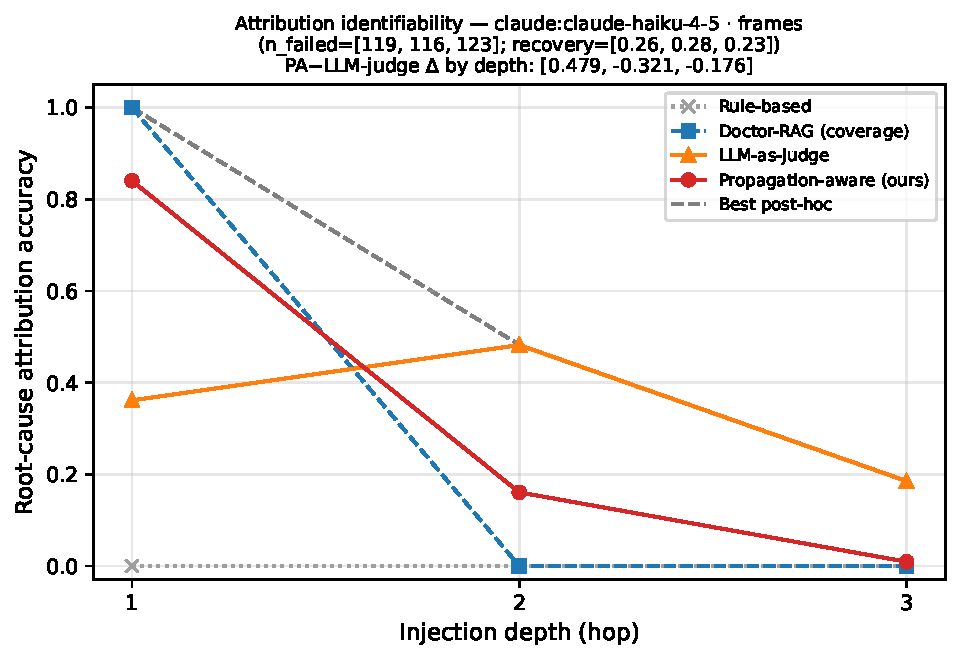
\includegraphics[width=0.48\linewidth]{identifiability_curve_claude_claude-haiku-4-5_frames.pdf}
\hfill
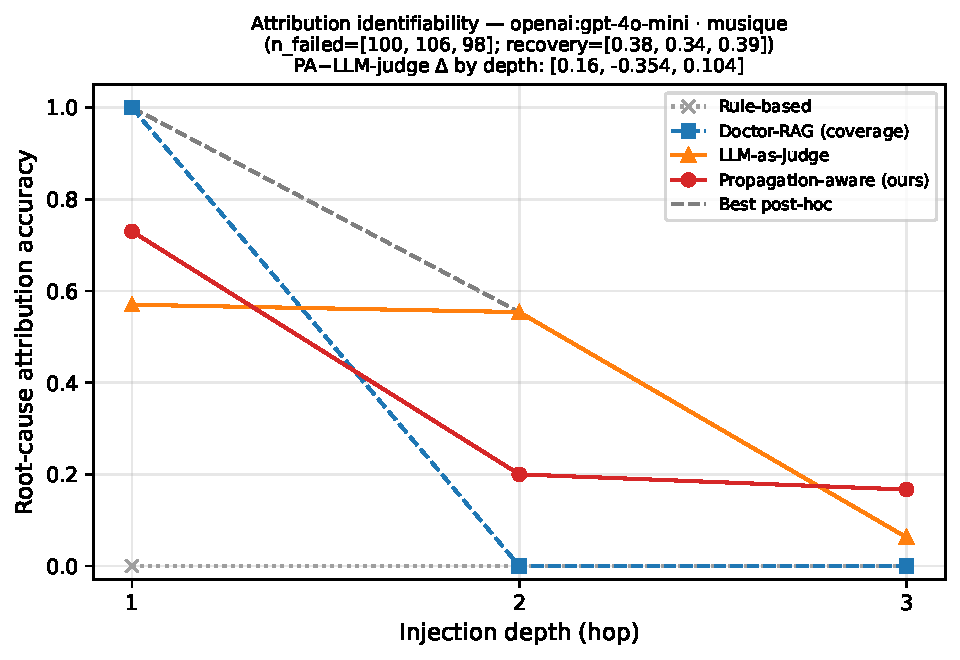
\includegraphics[width=0.48\linewidth]{identifiability_curve_openai_gpt-4o-mini_musique.pdf}
\caption{Representative attribution-identifiability curves (strict-rescored:
only cases whose actual injected hop equals the requested depth).  Left:
Claude Haiku 4.5 on FRAMES with BM25.  Right: GPT-4o-mini on MuSiQue with
BM25.  Each curve reports exact-hop attribution accuracy among injected traces
that remain failed after live suffix re-execution; depths with no failed cases
are omitted rather than plotted as zero.}
\label{fig:curves}
\end{figure}

\subsection{C3: Counterfactual Local Repair is Mixed}

The \pa{} diagnoser was designed to recover causal roots that post-hoc methods
cannot see.  The current exact-hop evidence does not support this as a general
claim.  Table~\ref{tab:c3-verdict} summarizes the depth-$\geq 2$ comparison
against the best post-hoc baseline.

\begin{table}[t]
\centering
\small
\begin{tabular}{p{0.43\linewidth}ccc}
\toprule
Evaluation slice & Conditions & \pa{} wins & Interpretation \\
\midrule
Depth $\geq 2$, structural, decontaminated & 6 & 0 & Not supported \\
Depth $\geq 2$, content faults, vs \dr{} & 4 & 4 & Supported vs coverage \\
Depth $\geq 2$, content faults, vs best post-hoc & 4 & 0 & \lj{} envelope wins$^\ast$ \\
\bottomrule
\end{tabular}
\caption{C3 verdict after decontamination.  On structural faults \pa{} never
beats the best post-hoc envelope at depth (an earlier 3-of-13 count reflected
contaminated buckets).  On content faults it decisively beats coverage gating
(0.67 vs.\ 0.00 pooled at hop 2) but not the judge-inclusive envelope.
$^\ast$The judge's deep advantage is partly a mid-trace prior
(\S\ref{sec:judge-robust}).}
\label{tab:c3-verdict}
\end{table}

Table~\ref{tab:dense-openai} shows the strengthened dense GPT-4o-mini runs with
larger sample size and probe budget 4, after decontamination.  The corrected
picture is starker than the loose numbers suggested: \dr{} retains nothing at
depth on either dataset, \lj{} is the strongest deep post-hoc method, and \pa{}
sits between them.

\begin{table}[t]
\centering
\small
\begin{tabular}{llcccc}
\toprule
Dataset & Depth & \dr{} & \lj{} & \pa{} & $n$ (strict) \\
\midrule
\multirow{3}{*}{HotpotQA, dense}
  & 1 & 1.00 & 0.35 & 0.61 & 75 \\
  & 2 & 0.00 & 0.58 & 0.36 & 33 \\
  & 3 & 0.00 & 0.50 & 0.30 & 20 \\
\midrule
\multirow{3}{*}{MuSiQue, dense}
  & 1 & 1.00 & 0.50 & 0.61 & 120 \\
  & 2 & 0.00 & 0.67 & 0.38 & 61 \\
  & 3 & 0.00 & 0.36 & 0.43 & 47 \\
\bottomrule
\end{tabular}
\caption{Strengthened GPT-4o-mini dense results, criterion = exact hop,
decontaminated (only cases whose actual injected hop equals the requested
depth; $n$ is the strict per-depth count of failed cases).  Per-depth recovery
rates are omitted here because the persisted per-depth recovery in pre-fix
files mixes clamped cases; fresh strict runs will restore them.}
\label{tab:dense-openai}
\end{table}

\subsection{C4: Content Corruption --- Total Coverage Collapse, Deterministic Absorption}
\label{sec:content-results}

Structural interventions are detectable by construction: an empty or off-topic
hop has near-zero coverage, so a coverage gate localizes it without any real
diagnostic skill.  The content-corruption arm removes this crutch.
Table~\ref{tab:content-acc} reports exact-hop accuracy pooled over the four
backbone--dataset conditions, restricted to injected traces that still fail
(bootstrap 95\% CIs, $B{=}1{,}000$); Figure~\ref{fig:corruption-curves} shows
the per-backbone HotpotQA curves.

\begin{table}[t]
\centering
\small
\begin{tabular}{lccc}
\toprule
Diagnoser & Hop 1 ($n{=}44$) & Hop 2 ($n{=}18$) & Hop 3 ($n{=}3$) \\
\midrule
\dr{} (coverage)      & 1.00 [1.00, 1.00] & 0.00 [0.00, 0.00] & 0.00 \\
\lj{} (cross-family)  & 0.59 [0.43, 0.73] & 0.89 [0.72, 1.00]$^\dagger$ & 0.33 \\
\pa{}                 & 0.89 [0.80, 0.98] & \textbf{0.67} [0.44, 0.89] & 0.00 \\
\sr{}                 & 0.91 [0.82, 0.98] & 0.11 [0.00, 0.28] & 0.00 \\
\bottomrule
\end{tabular}
\caption{Exact-hop attribution on \emph{content} faults, pooled over
\{GPT-4o-mini, Claude Haiku 4.5\} $\times$ \{HotpotQA, MuSiQue\} (BM25,
$n{=}40$ per condition, strict eligibility).  Coverage gating collapses
totally at depth 2; the counterfactual \pa{} probe holds.  $^\dagger$Partly a
mid-trace prior; see \S\ref{sec:judge-robust}.  Hop-3 cells have $n{=}3$ and
are indicative only.}
\label{tab:content-acc}
\end{table}

Three results stand out.  \textbf{First}, the coverage collapse is \emph{total}
on content faults: \dr{} falls from 1.00 to 0.00 with a degenerate bootstrap
interval, sharper than the 0.93$\rightarrow$0.30 structural-arm aggregate.
Even its hop-1 perfection is partly gifted --- answer-fact corruption removes
the gold string from the documents, so the gold-coverage gate fires; bridge and
salient corruptions leave the gate to default to hop 1.  \textbf{Second}, \pa{}
retains 0.67 at depth 2 where coverage retains nothing --- the clearest
depth-$\geq 2$ advantage for counterfactual probing in any of our conditions,
and the C3 signal the structural arm failed to produce.  Sliced by corruption
strategy, this advantage concentrates in answer-fact corruption (1.0 / 0.6 /
0.75 at hop 2 across conditions).  \textbf{Third}, \sr{} collapses at depth 2
(0.11) for a mechanistic reason: after repairing hop $h$, it regenerates the
suffix by re-retrieving from the \emph{clean} corpus, which silently
un-corrupts a deeper injected fault --- flipping the outcome while probing
hop 1 and thus systematically under-localizing.  \pa{}, which freezes all other
hops, is immune to this.  Conversely, \sr{} wins the bridge-entity slice (1.00
vs.\ \pa{} 0.73, $n{=}11$), where downstream hops were derived from the
corrupted bridge and \emph{must} be regenerated for the repair to register.
The two probes fail in complementary regimes, which directly motivates a
cascaded diagnoser.

\paragraph{Absorption.}
Table~\ref{tab:absorption} reports the deterministic generation-level
classification over \emph{all} injected cases (not only failures).

\begin{table}[t]
\centering
\small
\begin{tabular}{lcccc}
\toprule
Depth & Absorbed & Resisted & Derailed & $n$ \\
\midrule
Hop 1 & 0.15 & 0.58 & 0.26 & 106 \\
Hop 2 & 0.09 & 0.74 & 0.18 & 68 \\
Hop 3 & 0.00 & 0.85 & 0.15 & 20 \\
\bottomrule
\end{tabular}
\caption{Deterministic absorption classification of generated answers against
certified corruption spans, pooled over the four content-corruption
conditions.  Hop-1 absorbed rates are backbone-stable (0.18 / 0.19 / 0.11 /
0.11 across the four conditions).}
\label{tab:absorption}
\end{table}

\begin{figure}[t]
\centering
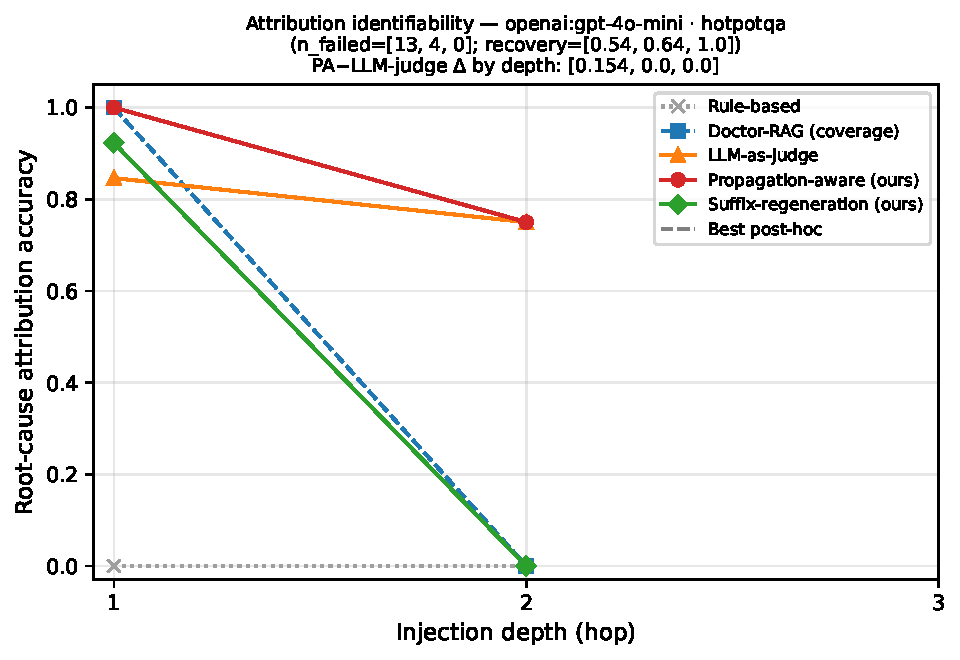
\includegraphics[width=0.48\linewidth]{identifiability_curve_openai_gpt-4o-mini_hotpotqa_bm25_corruption.pdf}
\hfill
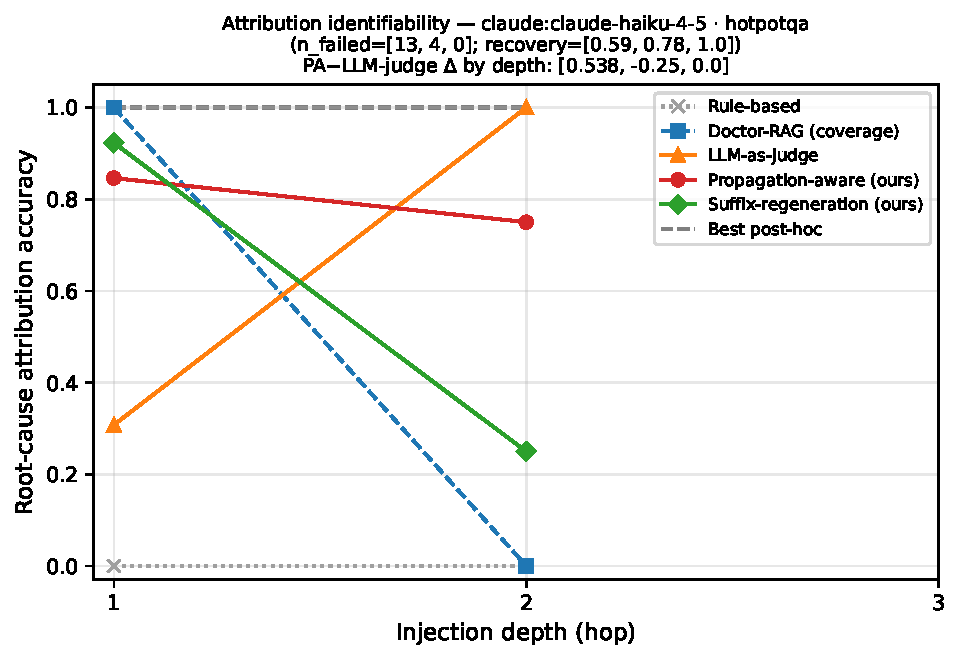
\includegraphics[width=0.48\linewidth]{identifiability_curve_claude_claude-haiku-4-5_hotpotqa_bm25_corruption.pdf}
\caption{Content-corruption identifiability curves on HotpotQA (BM25, strict
protocol).  Left: GPT-4o-mini agent (Claude Haiku 4.5 judge).  Right: Claude
Haiku 4.5 agent (GPT-4o-mini judge).  Coverage gating (\dr) and
suffix-regeneration collapse to zero at hop 2 while the frozen-hop
counterfactual probe (\pa) holds 0.75 on both backbones; hop 3 is omitted
where no injected trace remained failed (high recovery).}
\label{fig:corruption-curves}
\end{figure}

Absorption is almost exclusively \emph{answer-shaped}: 20 of 22 absorbed cases
are answer-fact corruptions, while salient-entity corruptions are never
absorbed (0 of 40) --- when the corrupted value looks like an answer, the agent
repeats it; when it is a chain link, corruption derails rather than misleads.
Query contamination is near zero (3 of 129 cases): corrupted values propagate
through the agent's \emph{reasoning} into the answer, not through its re-query
text, so monitoring sub-queries alone would miss essentially all content-fault
propagation.  Finally, recovery on content faults (0.54--0.85) is far higher
than on structural faults (0.00--0.71): the trajectory is corrupted but the
corpus stays clean, so re-retrieval heals.  This is the faithful
trajectory-level $do()$ operator, but it bounds how often deep content faults
survive to be diagnosed; a persistent-corruption variant that also corrupts
the corpus copy (the stale-index model) is the natural follow-up.

\subsection{LLM-Judge Depth-Robustness is Partly a Mid-Trace Prior}
\label{sec:judge-robust}

Across decontaminated conditions, \dr{} drops to zero at depth while \lj{} is
comparatively flat.  For example, on Claude MuSiQue dense, \dr{} drops from
1.00 to 0.00 by hop 2, whereas \lj{} rises from 0.16 to 0.80.  On OpenAI
FRAMES dense, \dr{} drops from 0.98 to 0.03 by hop 2, whereas \lj{} remains
around 0.64.  This suggests that reasoning over the full trajectory can be
more robust to propagation than simple gold-answer coverage, although it
incurs token cost and can still mislocalize.

The content-corruption arm, however, reveals that part of this robustness is an
artifact.  Inspecting the judge's predicted-hop distribution shows that at
depth 2 it predicts ``hop 2'' almost unconditionally (12 of 14 failed cases
pooled), while at depth 1 its predictions scatter (on Claude HotpotQA traces:
six abstentions and predictions ranging over hops 1--4, yielding 0.36
accuracy).  A diagnoser with a fixed mid-trace prior scores well at depth 2 by
construction.  The judge's depth-robustness should therefore be read as an
upper bound that mixes genuine trajectory reasoning with prior-matching; the
cross-family judging in this arm rules out self-recognition but not this
positional bias.

\subsection{Recovery is a First-Class Outcome}

Table~\ref{tab:recovery} shows selected counterfactual recovery rates.  Recovery
is computed before filtering failed traces for attribution.  This makes it a
separate robustness axis: high recovery means the injected fault did not cause a
final error.

\begin{table}[t]
\centering
\small
\begin{tabular}{p{0.58\linewidth}ccc}
\toprule
Condition & Hop 1 & Hop 2 & Hop 3 \\
\midrule
OpenAI GPT-4o-mini, HotpotQA, dense & 0.69 & 0.69 & 0.71 \\
OpenAI GPT-4o-mini, MuSiQue, dense & 0.50 & 0.53 & 0.56 \\
OpenAI GPT-4o-mini, FRAMES, dense & 0.20 & 0.18 & -- \\
Claude Haiku 4.5, FRAMES, BM25 & 0.26 & 0.28 & 0.23 \\
Qwen2.5:7B, MuSiQue, BM25 & 0.25 & 0.20 & 0.17 \\
\bottomrule
\end{tabular}
\caption{Counterfactual recovery by depth for selected conditions.  Agents can
often absorb retrieval faults, especially on HotpotQA, while FRAMES remains
fragile.  Per-depth values from pre-fix files include clamped cases at the
labeled depth and should be read as approximate; overall recovery levels are
unaffected.}
\label{tab:recovery}
\end{table}

\subsection{Static Control: Propagation Masks Retrieval Roots}

The static ablation grid gives a deterministic control over HotpotQA and
MuSiQue with BM25 and token-overlap retrievers.  It shows the same masking
pattern in a simpler setting.  On BM25 HotpotQA, empty retrieval at hop 1 is
diagnosed as retrieval with root-cause accuracy 1.00, but empty retrieval at
hops 2 and 3 is diagnosed as answer-generation failure with root-cause accuracy
0.00.  On BM25 MuSiQue, the pattern repeats: hop-1 empty retrieval has
root-cause accuracy 1.00, while hops 2 and 3 have 0.00.  The static propagation
graph estimates retrieval-to-answer coupling of 0.82 on HotpotQA and 0.94 on
MuSiQue for empty retrieval.

\begin{figure}[t]
\centering
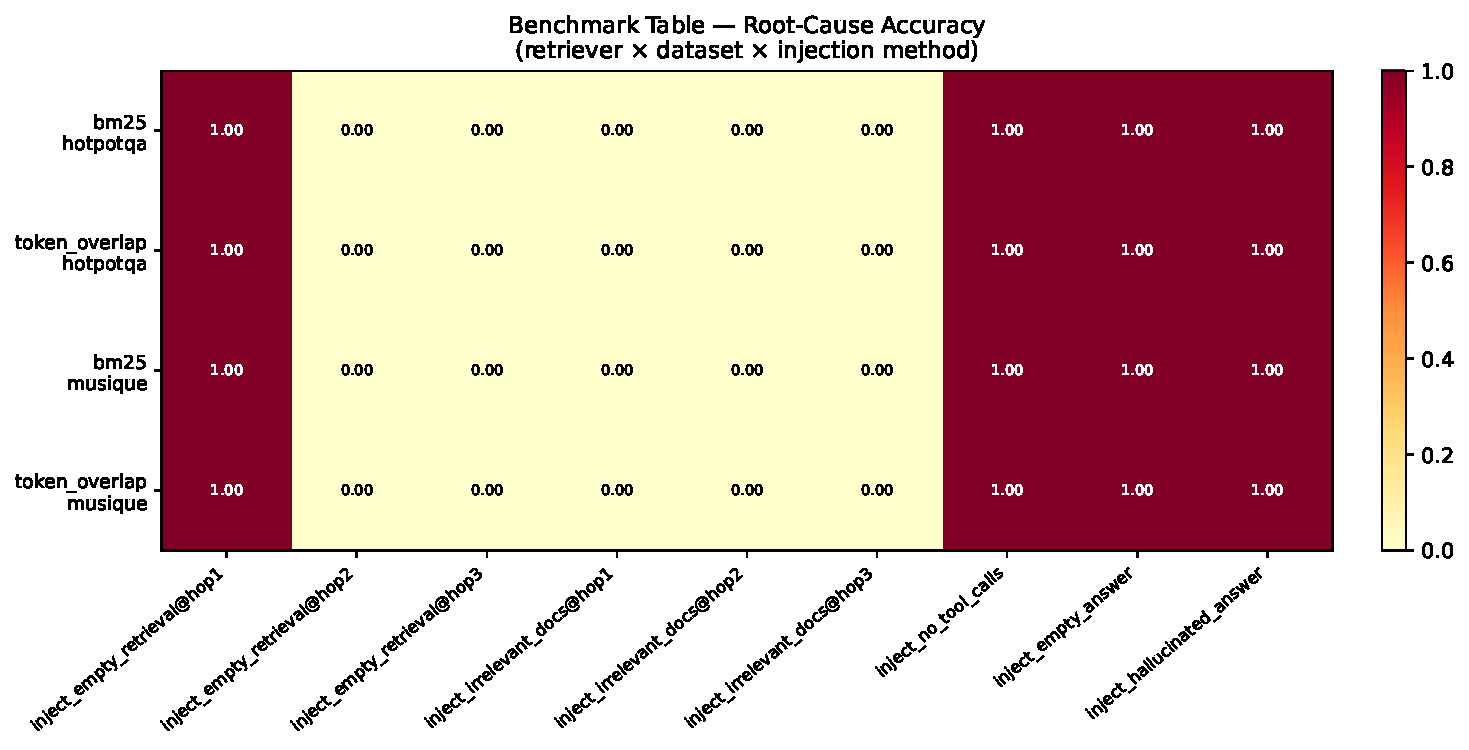
\includegraphics[width=0.72\linewidth]{benchmark_table_root_cause_accuracy.pdf}
\caption{Generated benchmark table for root-cause accuracy in the static
ablation suite.  Static controls are not the headline causal experiment, but
they provide a cheap regression test for propagation masking.}
\label{fig:static-table}
\end{figure}

\section{Discussion}
\label{sec:discussion}

\paragraph{Why coverage collapses.}
Coverage gating assumes that the earliest hop with low answer support is the
root cause.  This assumption holds when faults manifest locally: an empty
retrieval at hop 1 immediately produces low coverage at hop 1, and the agent
does not recover.  It breaks once the agent re-runs the downstream suffix,
because later hops can mask the original fault by retrieving compensatory
evidence or propagate it by issuing queries already biased by the corrupted
context.  In either case, the final trace no longer carries a reliable signature
of the injected hop.  The observed collapse is therefore an
\emph{identifiability limit}---a structural property of the signal available
to post-hoc methods---not merely a weak implementation.

\paragraph{Why the current \pa{} method underperforms.}
The \pa{} probe repairs one hop at a time and forces an answer from the modified
hop sequence, holding all remaining hops fixed.  This is causally motivated, but
it is a weak localizer when downstream artifacts depend on the original fault.
Repairing hop $h$ while holding later corrupted hops fixed may not flip the
answer even when $h$ was the true cause, because the later hops were themselves
generated from the corrupted prefix.  Conversely, repairing a later
answer-bearing hop can flip the outcome and steal credit from the true earlier
cause.  This explains the gap between exact-hop scoring and the looser stage
criterion: \pa{} often identifies the broad failure stage correctly (e.g., the
agent halted at retrieval failure) but cannot isolate the exact injected hop.

\paragraph{Implications for repair.}
\label{sec:implications}
The negative C3 result is useful.  It suggests that deployable repair should not
only ask ``which hop flips if repaired?'' but should model paths of downstream
dependence.  Our \sr{} diagnoser (\S\ref{sec:diagnosers}) implements one such
path: it regenerates the downstream suffix after repairing hop $h$, rather than
forcing an answer from the frozen corrupted later hops.  Its first evaluation
(\S\ref{sec:content-results}) shows the two probes fail in \emph{complementary}
regimes rather than one dominating: \sr{} wins exactly where its design
predicts --- bridge-entity corruption, where downstream hops derive from the
corrupted prefix and must be regenerated (1.00 vs.\ \pa{} 0.73) --- but
collapses on deep answer-fact corruption (0.11 at depth 2 vs.\ \pa{} 0.67)
because regenerating the suffix re-retrieves clean evidence and un-corrupts the
very fault being probed.  This argues for a \emph{cascaded} diagnoser that
selects the probe by suspected fault type (or runs a cheap judge first and a
targeted counterfactual probe second), rather than a single universal probe.
Other candidate improvements include multi-hop repair sets, explicit
query-drift detection, and confidence-calibrated abstention when multiple hops
are causally entangled.

\section{Limitations}

First, several result files are partial or unrescoreable.  Dense Claude
HotpotQA currently contains only hop 1; dense Claude MuSiQue contains hops
1--2; four early conditions did not persist raw diagnoses and are excluded
from depth-specific claims entirely.  Depth decontamination removes clamping
but cannot retroactively apply base-correctness filtering, so injections into
already-failing base traces remain in the rescored pre-fix numbers; fresh
strict runs are required for final figures.

Second, scoring uses exact-hop localization as the strict headline criterion.
Stage-level diagnosis is easier and yields qualitatively different conclusions
for \pa{}: stage accuracy is consistently higher, indicating that \pa{} often
identifies the correct failure stage without pinpointing the exact hop.  Both
criteria are reported, and readers should attend to which criterion is relevant
for their use case.

Third, the mock provider is only a deterministic control, not a model of real
LLM reasoning.  Mock-based ablations test infrastructure but cannot substitute
for real-backbone identifiability experiments.

Fourth, LLM-as-judge results are sensitive to prompt design and token cost.
The current \lj{} prompt instructs the judge to report the earliest failing
hop and stage; alternative prompt designs could change the localization
behavior, and token cost makes large-scale use expensive.

Fifth, the dataset adapters rely on available supporting documents or fetched
Wikipedia passages, so corpus construction quality affects both intervention and
recovery rates.  The current runner records actual injected hops and skips short
base traces by default; older persisted result files should be rescored with
actual-depth filtering or regenerated before making final depth-specific claims.
The FRAMES corpus relies on Wikipedia passage fetching; runs without
\texttt{--frames-fetch-passages} use bare link title text as the retrieval
corpus, which inflates both recovery and identifiability scores relative to real
passage retrieval.  This is now detected automatically via
\texttt{corpus\_quality.link\_only\_fraction} and warned at run time.
Exact-hop accuracy CIs reported in this paper use bootstrap resampling ($B =
1{,}000$, seeded); low-$n$ conditions (CRAG, $n < 10$) have wide CIs that
should be read cautiously.

Sixth, the content-corruption arm corrupts the \emph{trajectory} copy of the
documents while the corpus stays clean --- the faithful trajectory-level
$do()$ operator, consistent with the structural interventions, but it lets
re-retrieval heal the fault.  Consequently recovery is high (0.54--0.85) and
the number of failed cases at depth $\geq 2$ is small ($n{=}18$ at hop 2,
$n{=}3$ at hop 3, pooled), so deep-depth comparisons in
Table~\ref{tab:content-acc} are indicative rather than statistically
significant.  A persistent-corruption variant (corrupting the corpus copy,
modeling a stale or poisoned index) and larger $n$ are required before
headline claims at depth 3.  Relatedly, the discordant-pair comparison of
\pa{} against the best post-hoc \emph{envelope} at depth $\geq 2$ (1 vs.\ 6
pairs) is too small for a McNemar test; the claim we make is \pa{} vs.\
coverage gating specifically, not \pa{} vs.\ all post-hoc methods.

\section{Conclusion}

\ours{} turns agentic RAG failure analysis into an intervention problem.  By
injecting faults at known hops and re-running the downstream suffix, it separates
three phenomena that end-to-end accuracy conflates: whether a fault causes a
final failure, whether the agent recovers, and whether a diagnoser can recover
the certified root cause.  The current experiments strongly support the
identifiability-collapse claim --- after depth decontamination, coverage gating
retains nothing at depth $\geq 2$ on structural \emph{and} content faults,
while counterfactual probing retains 0.67 on content faults at hop 2 --- and
show substantial counterfactual recovery.  The certified content-corruption
arm additionally contributes a deterministic, judge-free generation evaluation:
15\% of hop-1 corruptions are absorbed verbatim, absorption is answer-shaped,
and propagation flows through reasoning rather than re-query text.  Structural
faults did not support a broad exact-hop advantage for the propagation-aware
diagnoser, and the suffix-regeneration results explain why no single probe
suffices: local repair and suffix regeneration fail in complementary regimes.
The next version of the method should treat propagation as a path-localization
problem --- selecting the probe by suspected fault type --- rather than a
single-hop repair probe.

\bibliographystyle{plainnat}
\bibliography{references}

\appendix

\section{Implementation Notes}
\label{app:impl}

The core repository files corresponding to the paper are:
\begin{itemize}[leftmargin=*]
  \item \texttt{src/agenticrag/core.py}: trace schema, failure taxonomy,
  heuristic pipeline, and rule-based diagnostic benchmark.
  \item \texttt{src/agenticrag/agents.py}: provider-agnostic resumable LLM
  agent and token accounting.
  \item \texttt{src/agenticrag/injection.py}: static and live interventions.
  \item \texttt{src/agenticrag/corruption.py}: certified content corruption ---
  span selection, seeded replacement, and the deterministic
  absorbed/resisted/derailed classifier.
  \item \texttt{src/agenticrag/diagnosers.py}: rule-based, coverage-gated,
  LLM-judge, propagation-aware, and suffix-regeneration diagnosers.
  \item \texttt{src/agenticrag/datasets.py}: dataset adapters plus
  \texttt{frames\_corpus\_stats} for FRAMES corpus quality validation.
  \item \texttt{src/agenticrag/experiment.py}: ablation and identifiability
  runners with checkpointing.
  \item \texttt{src/agenticrag/evaluate.py} and
  \texttt{src/agenticrag/propagation.py}: metrics, bootstrap CIs, softer
  localization metrics, and propagation graph.
  \item \texttt{scripts/summarize\_identifiability.py}: post-hoc summary of
  result JSONs, computing best-post-hoc baselines, PA vs.\ LLM-judge deltas,
  bootstrap CIs, and per-intervention-type slices.
\end{itemize}

\section{Reproduction Commands}
\label{app:repro}

\begin{verbatim}
# Offline smoke:
python scripts/run_identifiability.py --dataset frames --provider mock \
  --retriever bm25 --hops 1 2 3

# Real-backbone identifiability:
python scripts/run_identifiability.py --dataset musique --provider openai \
  --model gpt-4o-mini --retriever dense --max-samples 60 \
  --hops 1 2 3 --propagation-budget 4 --tag dense_b4 --resume

# Static controls:
python scripts/run_baseline.py --all-conditions --max-samples 500
python scripts/run_ablation.py --all-conditions --max-samples 200 --hops 1 2 3

# Figures:
python scripts/plot_identifiability.py
python scripts/plot_amplification.py --input results/ablation_all.json

# Generate summary tables (best post-hoc, PA vs LLM-judge, slices, CIs):
python scripts/summarize_identifiability.py \
  --write-md results/RESULTS_SUMMARY.md --criterion hop

# Plots now show LLM-judge as primary comparator + best-posthoc envelope:
python scripts/plot_identifiability.py

# Content-corruption arm (certified spans, deterministic absorption eval,
# cross-family judge, suffix_regen included):
python scripts/run_identifiability.py --dataset hotpotqa --provider openai \
  --model gpt-4o-mini --retriever bm25 --max-samples 40 --hops 1 2 3 \
  --injection-methods inject_corrupted_evidence \
  --diagnosers rule_based doctor_rag llm_judge propagation_aware suffix_regen \
  --judge-provider claude --judge-model claude-haiku-4-5 \
  --tag bm25_corruption --resume
\end{verbatim}

\section{Additional Current Results}
\label{app:results}

The generated \texttt{results/RESULTS\_SUMMARY.md} contains the full current
condition table.  Selected decontaminated (strict actual-depth) deep
comparisons:
\begin{itemize}[leftmargin=*]
  \item Exact-hop: \pa{} beats the best post-hoc envelope in 0 of 6
  rescorable structural deep conditions (\lj{} is the strongest deep post-hoc
  method in every one); \pa{} beats \dr{} coverage in all of them, since \dr{}
  is 0.00 at depth everywhere.  Earlier per-condition win claims were computed
  on contaminated buckets and are superseded.
  \item Stage-criterion rescoring (strict) remains much more favorable to
  \pa{} at depth $\geq 2$: 0.96--1.00 on Claude FRAMES BM25, 0.91 on Claude
  MuSiQue dense, 0.87 on OpenAI FRAMES dense, 0.82--0.83 on OpenAI MuSiQue
  BM25, 0.69--0.70 on OpenAI MuSiQue/HotpotQA dense --- versus 0.16--0.43
  hop-exact.  \pa{} reliably identifies the broad failure stage but not the
  exact injected hop; hierarchical (stage $\rightarrow$ hop) localization is
  the honest report of what counterfactual probing currently delivers.
\end{itemize}

\end{document}
